\chapter{Nuclear dependence of antineutrino cross-section}

%It enables a direct comparison of the impact of nuclear effects on antineutrino scattering, as well as the strong dynamics of the nucleon and nucleus that affect these interactions. 
\vspace{-10pt}
\label{ch:measurement}
This thesis presents the first high-statistics simultaneous measurement of charged-current inclusive muon antineutrino differential cross-sections on carbon, hydrocarbon, iron, and lead as a function of antimuon transverse momentum $p_{\text{T}}$ and Bjorken $x$. Inclusive analysis in this case refers to an analysis considering all final states, i.e., all antineutrino interaction modes. The measurement uses data taken by the MINERvA experiment with peak antineutrino energy of~$\sim$6~GeV. It enables a direct comparison of the impact of nuclear effects in antineutrino scattering since the cross-sections are extracted employing identical techniques, within the same detector, and with the same antineutrino beam. Additionally, this measurement expands the antineutrino data sets, which are crucial for studying CP violation. 

This chapter focuses on the specific motivation for such measurement, as well as the general process of extracting the cross-section in the variables of interest. The data and the simulation sample, their reconstruction, and the analysis procedure itself are detailed in the subsequent chapters.


\section{Motivation for the measurement}

In 2014, MINERvA presented its first EMC-like measurement of inclusive charged-current neutrino scattering on carbon, hydrocarbon, iron and lead taken during the low-energy regime with peak neutrino energy of $\sim$3~GeV \cite{Tice_PhysRevLett.112.231801}. The cross-section ratios of iron-to-hydrocarbon and lead-to-hydrocarbon as a function of reconstructed Bjorken $x$ are shown in Figure~\ref{fig:emcLike}, exhibiting relative depletion at low $x$ and enhancement at large $x$, neither of which are predicted by the simulation prediction. These discrepancies increase with the size of the nucleus. At low $x$, the result suggested that the shadowing model based on charged-lepton scattering used in the prediction does not capture the shadowing in neutrino scattering well, and larger suppression may be required. The disagreement at high~$x$ was ascribed to the omission of multi-nucleon processes such as 2p2h in the simulation prediction.

\begin{figure}[b!]
    \centering
    \vspace{-5pt}
    {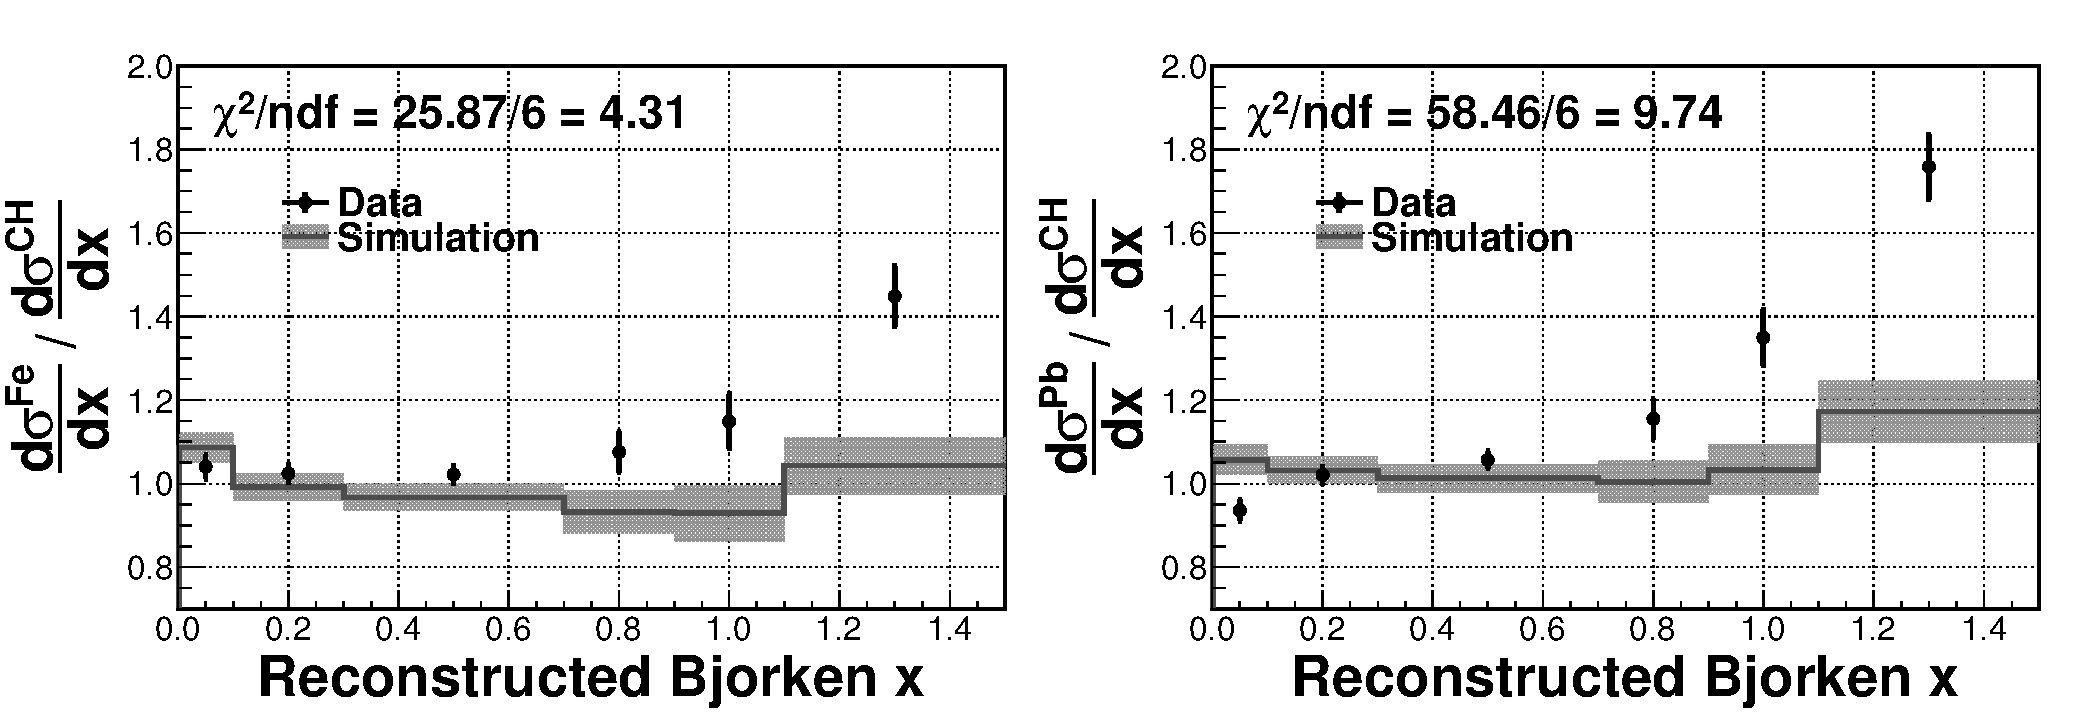
\includegraphics[width=1\textwidth]{04measurement/figures/emcLike.pdf}}%
    \vspace{5pt}
    \caption{MINERvA's measurement of iron-to-hydrocarbon (left) and lead-to-hydrocarbon (right) ratios of inclusive charged-current neutrino cross-sections per nucleon as a function of reconstructed Bjorken $x$. Reprinted with permission from Ref.~\cite{Tice_PhysRevLett.112.231801}. ~Copyright (2024) by the American Physical Society.}
    %[short caption] {long caption}
    \label{fig:emcLike}
\end{figure}

At the time, a similar analysis for inclusive antineutrino cross-section on different nuclear targets was impossible due to low statistics of antineutrino interactions in the low-energy sample. However, as a result of the long period of antineutrino operation of the NuMI beam in medium energy, MINERvA collected a high-statistics sample of antineutrino interactions that enables such investigation. Furthermore, the underlying simulation used in the measurement has undergone several improvements such as including the multi-nucleon scattering, possibly impacting the prediction for the high $x$ region. The full description of the simulation prediction used in the measurement presented in this thesis is included in Chapter~\ref{ch:dataAsimulation}. In addition, this analysis also benefits from improvements in the reconstruction of the interaction vertex crucial for distinguishing on which nucleus the interaction occurred, which are further elaborated on in Chapter~\ref{ch:Reconstruction}.

Notably, the 2014 neutrino analysis was also reported in terms of the reconstructed Bjorken~$x$ due to the inability to deconvolute the detector effects from the measurement \cite{TiceThesis2014}. Thanks to improvements in interaction modelling, reconstruction techniques, increased statistics in the sample, and rigorous unfolding studies (detailed in Section \ref{sec:migration_unfolding}), this medium-energy antineutrino analysis can now estimate the cross-section in terms of the true Bjorken $x$. This allows for reporting a detector-independent cross-section, which is valuable for interpretation in the context of various theoretical and phenomenological studies, as well as for comparisons with results from other experiments. Furthermore, the results are also reported in terms of the well-reconstructed antimuon transverse momentum $p_{\text{T}}$, which can be related to the four-momentum transfer squared in the interaction. 

% SRC

\begin{figure}[t!]
    \centering
    {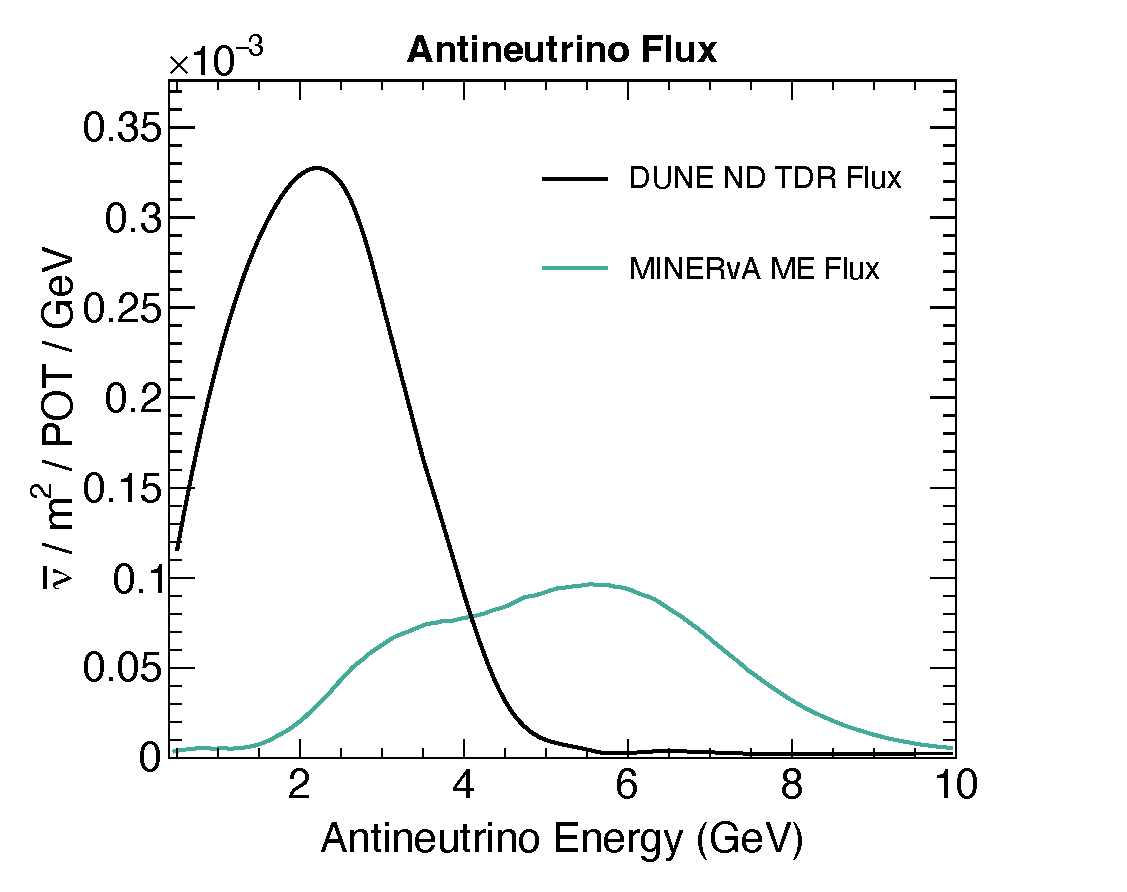
\includegraphics[width=0.75\textwidth]{04measurement/figures/antinu_flux.pdf}}%
    \caption{Comparison of the expected antineutrino flux at the DUNE near detector~(ND) according to ND Technical Design Report (TDR)~\cite{abi2020deep} and the MINERvA medium energy antineutrino flux in the 0--10 GeV range of antineutrino energy.~Note the significant overlap at the upper end of antineutrino energy.}
    %[short caption] {long caption}
    \label{fig:fluxDune}
\end{figure}

Due to the kinematic phase space spanned by the MINERvA medium energy dataset, the measurement presented in this work is predicted to be dominated by the resonant pion production, deep inelastic scattering, and the transition region between these two interaction modes, i.e. the shallow inelastic scattering. Understanding of the (anti)neutrino interactions and the nuclear effects in this energy regime is particularly important for the future oscillation experiment DUNE. This is demonstrated in Figure~\ref{fig:fluxDune} showing the expected antineutrino flux seen by the DUNE near detector compared to the MINERvA medium energy antineutrino flux utilised in this analysis, with a significant overlap corresponding to the energies where these higher-energy interaction modes are expected (cf. Figure~\ref{fig:totalXsecEnu} in Chapter~\ref{ch:theory}). 

Importantly, the (anti)neutrino scattering in DUNE will occur primarily on argon \cite{abi2020deep}. While experiments measuring (anti)neutrino cross-sections on argon exist, e.g. MicroBooNE~\cite{Acciarri_2017}, they generally probe lower-energy regions dominated by the quasi-elastic scattering. MINERvA is the only experiment that can provide direct high-statistics measurements of nuclear dependence across various nuclei in the kinematic regime dominated by these higher-energy interaction modes. Therefore, MINERvA measurements, including this one, are crucial for refining our understanding and modelling of the impact that nuclear effects have on these interaction modes, enabling the interpolation to interactions on argon. The NOvA experiment \cite{NOVA_2005nova} is also able to study these interaction channels at slightly lower energies but on a scintillator only. 

More generally, this antineutrino measurement also expands the available antineutrino datasets in the energy regime relevant to the oscillation experiments, aiding in the refinement of antineutrino interaction modelling necessary for CP violation searches. Large antineutrino datasets are somewhat rare compared to their neutrino counterparts \cite{Workman:2022ynf}, primarily due to the extended time required for collecting antineutrino scattering data. This stems from the production process of the antineutrino beam, where negatively charged pions (that decay to antineutrinos) are less likely to be produced from the protons-carbon interactions \cite{numi2016_ADAMSON2016279}. Additionally, antineutrino cross-sections are lower than those for neutrinos, as shown in Figure~\ref{fig:totalXsecEnu}.



, and they predominantly span either the quasi-elastic (e.g. T2K) or the very high-energy deep inelastic region \cite{Workman:2022ynf}. %Measurements in the $1$ GeV $<E_\bar{\nu}> < 10 $ GeV have been made by for example by MINOS on iron, 
% https://pdg.lbl.gov/2023/reviews/rpp2022-rev-nu-cross-sections.pdf

\begin{figure}[t!]
    \centering
    {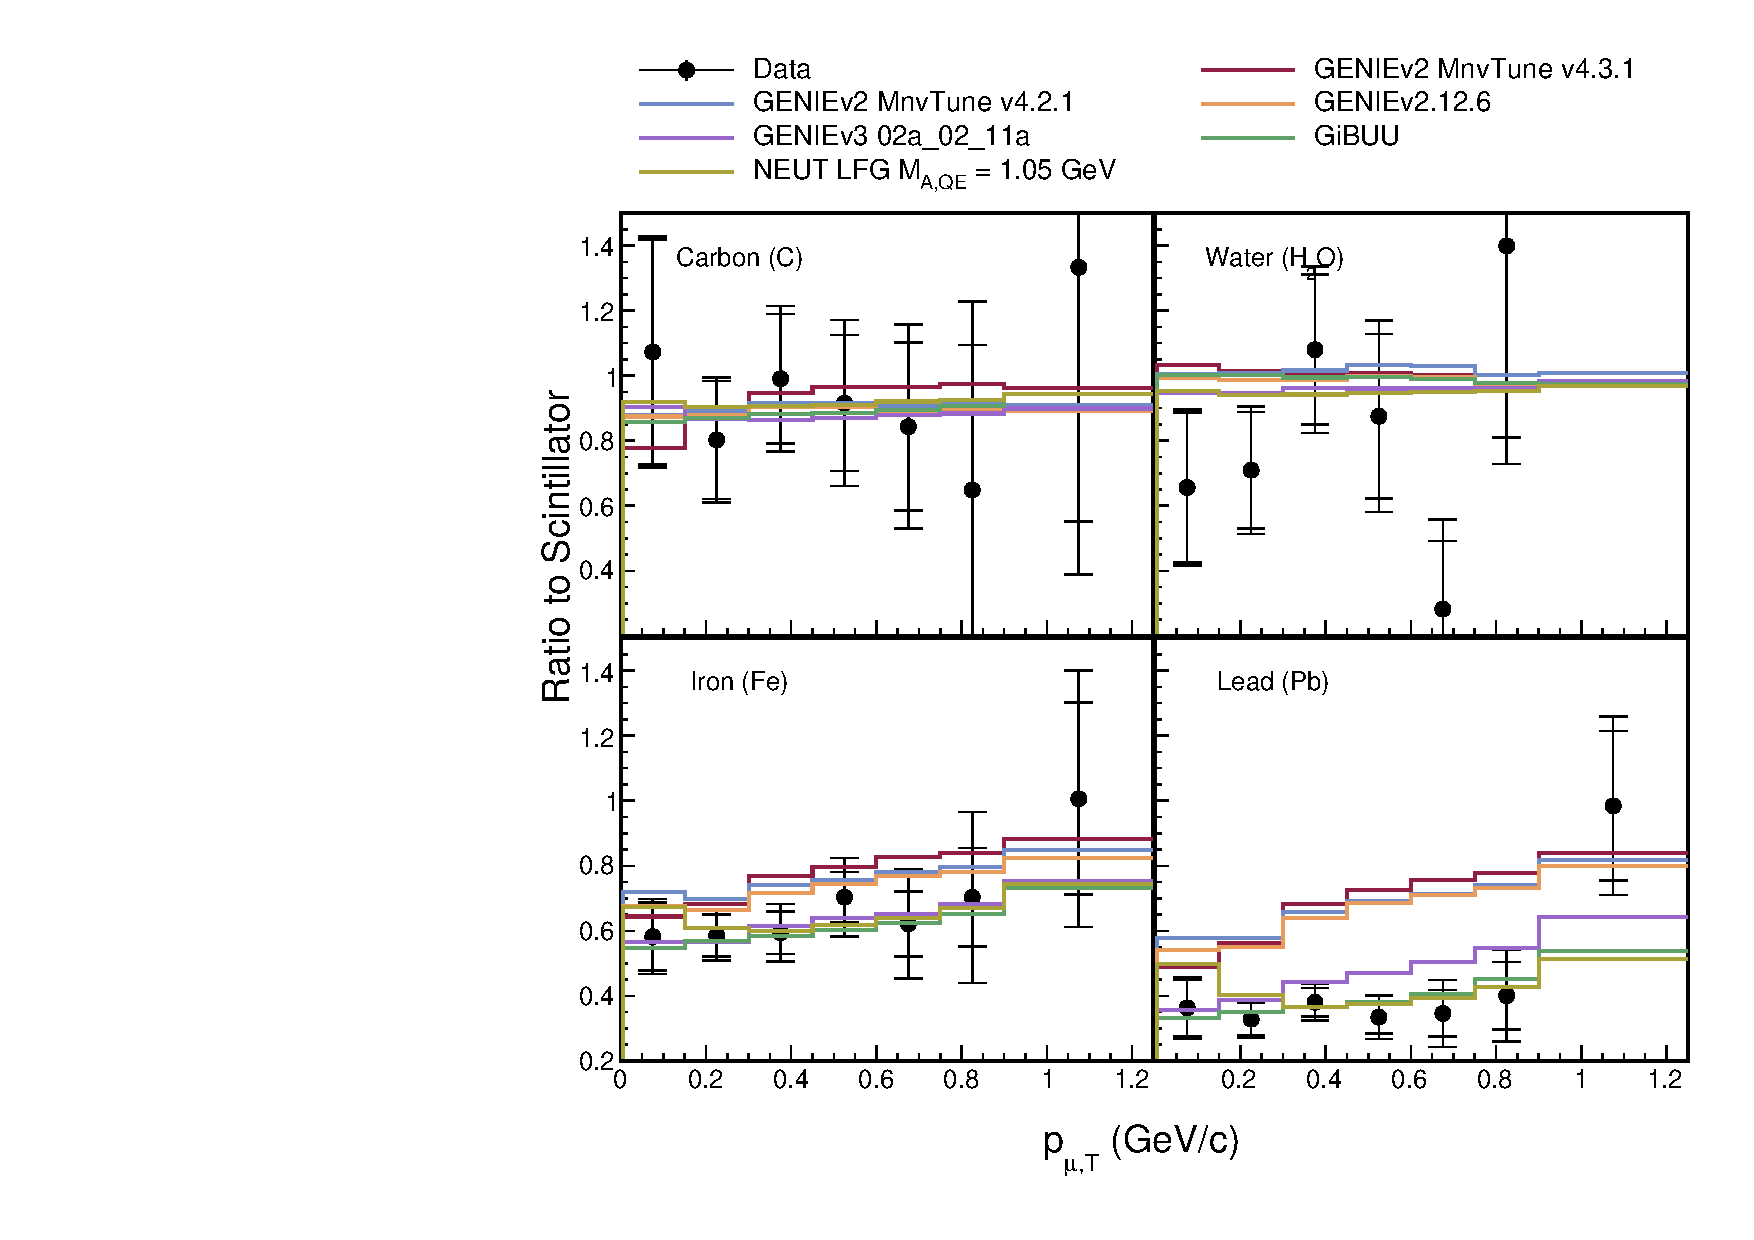
\includegraphics[width=0.8\textwidth]{04measurement/figures/aaronCC1pi.pdf}}%
    \vspace{5pt}
    \caption{MINERvA measurement of cross-section ratios for carbon, water, iron, and lead to the scintillator, i.e. hydrocarbon, for neutrino-induced charged-current single $\pi^+$ production in medium energy as a function of muon transverse momentum $p_{\text{T}}$ compared to various neutrino simulation predictions. Note that all of them are discrepant for either one or more nuclei with data showing low $p_{\text{T}}$ ($\sim Q^2$) suppression increasing with the size of the nucleus compared to the underlying simulation indicated by GENIEv2 MnvTune v4.3.1. Reprinted with permission from Ref.~\cite{Bercellie2023_PhysRevLett.131.011801}.~Copyright (2024) by the American Physical Society.}
    %[short caption] {long caption}
    \label{fig:aaronCC1pi}
\end{figure}

Finally, due to the dominant contribution from the single-pion production channel, this analysis allows for an inclusive investigation of the behaviour observed in MINERvA's measurement of neutrino-induced single-pion production across various nuclei \cite{Bercellie2023_PhysRevLett.131.011801}, as shown in Figure~\ref{fig:aaronCC1pi}, but in the antineutrino mode. 

% minerva medium energy of CC1pi + showed need for strong suppression at low Q^2 of
% this analysis enables its study in antineutrino mode


\section{How to measure the cross-section}
\begin{comment}

- MINERvA's medium energy analysis of charged-current single pion production showed a need for large suppression at low Q^2 
- see the need for a suppression of the
pion production prediction at low 𝑄2.

minerva run completed, but data continues to be analysed 
measurements help improve theoretical interaction models, essential components of neutrino oscillation programs
\end{comment}

The probability that a certain interaction process occurs is parameterised as a cross-section and can be thought of as the effective area subtended by the target particle to an incident beam \cite{perkins_2000}. This measurement reports flux-integrated differential cross-sections per nucleon on particular nuclei, namely carbon, hydrocarbon, iron, and lead. The cross-section distributions are discretised into a finite number of bins of a quantity of interest, defined in order to obtain a statistically significant sample in each of them, and are extracted as follows,
\begin{equation}
    \label{eq:xsec1D}
    {\left(\frac{d\sigma}{dx}\right)}_{\alpha} = \frac{\Sigma_{j} \tilde{U}_{j\alpha}(N_{\text{data}, j} - N^{\text{bkg}}_{\text{data}, j})}{E_{\alpha} T_{\text{nucleons}} \Phi \Delta x_{\alpha} \text{POT}} \hspace{2pt}.
\end{equation}

In the above, the left-hand side corresponds to the cross-section in bin $\alpha$ with respect to a quantity $x$. In this analysis, this quantity can either be antimuon transverse momentum $p_{\text{T}}$ or Bjorken~$x$.~To distinguish between the true value of the variable of interest, in which the final detector-independent cross-section is reported, and its reconstructed value, the bin containing the true value is labelled as $\alpha$, while the bin containing the reconstructed value is represented by $j$. The difference between the true bin and the reconstructed bin arises from the complex nature of the antineutrino interactions and the imperfect reconstruction, further explained in the following chapters.

$N_{\text{data}, j}$ is the number of reconstructed events of interest in bin $j$ and $N_{\text{data},j}^{\text{bkg}}$ is the estimated number of background events. The background-subtracted selected events correspond to the signal. Therefore, in this analysis, it is the number of all charged-current antineutrino interactions that occurred in a specific target material with certain kinematic constraints discussed in Chapter~\ref{ch:analysis1D}. $\tilde{U}_{j\alpha}$ represents the so-called unfolding process which tries to
remove the smearing of the reconstructed distribution to report the cross-section in the true quantities $\alpha$. Efficiency correction $\epsilon_{\alpha}$ takes into account the signal events that were lost due to detector acceptance and imperfect reconstruction. 

Furthermore, the differential cross-section is normalised to the flux prediction integrated over all bins, $\Phi$, the number of nucleons in a given material, $T_{\text{nucleons}}$, the bin width of the corresponding bin, $\Delta x$, to make it differential, and the number of protons on the target, POT, which is the metric used to characterize the integrated luminosity of the antineutrino beam. Note that all these individual steps of the cross-section extraction are described in detail in Chapter~\ref{ch:analysis1D}.

Finally, similar to the MINERvA analysis in Figure~\ref{fig:emclike}, the cross-section ratios of the nuclear target (A) to scintillator tracker (CH) are reported to minimise the dependence on the underlying antineutrino flux, as well as to cancel out some shared reconstruction and antineutrino interaction modelling effects. While the cross-section ratios are taken directly from the calculated cross-sections according to Equation~\ref{eq:xsec1D}, the ratios approximately correspond to
\vspace{-5pt}
\begin{equation}
    \left( \frac{d\sigma^\text{A}}{dx} \mathlarger{\mathlarger{\mathlarger{/}}} \frac{d\sigma^{\text{CH}}}{dx} \right)_{\alpha} \approx \mathlarger{\sum_j} \frac{\tilde{U}_{\alpha j}^\text{A}(N_{\text{data}, j}^\text{A}- N_{\text{data},j}^{\text{bkg},\text{A}})\epsilon_{\alpha}^{\text{CH}}T^{\text{CH}}}{\tilde{U}_{\alpha j}^{\text{CH}}(N_{\text{data}, j}^{\text{CH}}- N_{\text{data},j}^{\text{bkg},\text{CH}})\epsilon_{\alpha}^{\text{A}} T^{\text{A}}} \hspace{2pt}.
    \label{xsecs_ratios}
\end{equation}

\section{Variables of interest}

The final cross-section and cross-section ratio results are reported in terms of the antimuon transverse momentum $p_{\text{T}}$ and Bjorken $x$. The muon transverse momentum variable is well-reconstructed and can be related to the four-momentum transfer. The Bjorken x variable directly considers hadronic final states and is used to describe nuclear modifications to a bound nucleon cross-section compared to a free nucleon

How to relate

\begin{comment}

- why important
- signal definition
- other analyses
- define muon pT
- define Bjorken x
- x greater than 1 region
- why cross-section ratios
\end{comment}
